\documentclass[12pt,a4paper]{article}  % Khai báo lớp văn bản
\usepackage[utf8]{vietnam} % Gói lệnh phông tiếng Việt
\usepackage{a4wide,amssymb,epsfig,latexsym,multicol,array,hhline,fancyhdr}

\usepackage{amsmath}
\usepackage{lastpage}
\usepackage[lined,boxed,commentsnumbered]{algorithm2e}
\usepackage{enumerate}
\usepackage{color}
\usepackage{graphicx}							
% Standard graphics package
\usepackage{array}
\usepackage{tabularx, caption}
\usepackage{multirow}
\usepackage{multicol}
\usepackage{rotating}
\usepackage{graphics}
\usepackage[a4paper,left=2cm,right=2cm,top=1.8cm,bottom=2.8cm]{geometry}
\usepackage{setspace}
\usepackage{epsfig}
\usepackage{tikz}
\usetikzlibrary{arrows,snakes,backgrounds}
\usepackage{csquotes}% chèn trích dẫn câu nói
	\DeclareQuoteStyle[american]{english}
	{\itshape\textquotedblleft}
	[\textquotedblleft]
	{\textquotedblright}
	[0.05em]
	{\textquoteleft}
	{\textquoteright}	
\usepackage[unicode]{hyperref}
	\hypersetup{urlcolor=blue,linkcolor=black,citecolor=black,colorlinks=true} 
	%\usepackage{pstcol} 								
	% PSTricks with the standard color package
	
	\newtheorem{theorem}{{\bf Theorem}}
	\newtheorem{property}{{\bf Property}}
	\newtheorem{proposition}{{\bf Proposition}}
	\newtheorem{corollary}[proposition]{{\bf Corollary}}
	\newtheorem{lemma}[proposition]{{\bf Lemma}}
\setlength{\headheight}{40pt}
\pagestyle{fancy}
%Tiêu đề phía trên
\fancyhead{} % clear all header fields
\fancyhead[L]{
	\begin{tabular}{rl}
		\begin{picture}(25,15)(0,0)
		\put(0,-8){
\includegraphics[width=8mm, height=8mm]{hcmut.png}}
		%\put(0,-8){\epsfig{width=10mm,figure=hcmut.eps}}
	   \end{picture}&
		%
\includegraphics[width=8mm, height=8mm]{hcmut.png} & %
		\begin{tabular}{l}
			\textbf{\bf \ttfamily Trường Đại học Bách Khoa, ĐHQG TP.Hồ Chí Minh}\\
			\textbf{\bf \ttfamily Khoa Khoa học \& Kĩ thuật Máy tính}
		\end{tabular} 	
	 \end{tabular}
	}
	\fancyhead[R]{
		\begin{tabular}{l}
			\tiny \bf \\
			\tiny \bf 
		\end{tabular}  }
	\fancyfoot{} % clear all footer fields
	\fancyfoot[L]{\scriptsize \ttfamily Ứng dụng thống kê - Khảo sát kết của bài tập online cho phép nộp bài nhiều lần}
	\fancyfoot[R]{\scriptsize \ttfamily Trang {\thepage}/\pageref{LastPage}}
	\renewcommand{\headrulewidth}{0.3pt}
	\renewcommand{\footrulewidth}{0.3pt}
%Trang bìa
%--------------------------------
\begin{document} 
\begin{titlepage}

	\begin{center}
	TRƯỜNG ĐẠI HỌC BÁCH KHOA, ĐHQG TP.HỒ CHÍ MINH\\
	KHOA KHOA HỌC \& KỸ THUẬT MÁY TÍNH
	\end{center}
	
	\vspace{1cm}
	
	\begin{figure}[h!]
	\begin{center}
	
\includegraphics[width=3cm]{hcmut.png}
	\end{center}
	\end{figure}
	
	\vspace{1cm}
	
	
	\begin{center}
	\begin{tabular}{c}
	\multicolumn{1}{l}{\textbf{{\Large BÁO CÁO BTL CẤU TRÚC RỜI RẠC CHO KHMT}}}\\
	~~\\
	\hline
	\\
	\multicolumn{1}{l}{\textbf{{\Large Ứng dụng Thống kê}}}\\
	\\
	\textbf{\normalsize \textit{ Khảo sát kết quả của bài tập online cho phép nộp bài nhiều lần}}\\
	\\
	\hline
	\end{tabular}
	\end{center}
	
	\vspace{3cm}
	
	\begin{table}[h]
	\begin{tabular}{rrl}
	
	\hspace{4 cm} & Giáo viên hướng dẫn: & Huỳnh Tường Nguyên\\
	& & Trần Tuấn Anh \\
	& & Nguyễn Ngọc Lễ  \\
	%& Class: MT19KH10, & Group: Groove Street \\
	& Thành viên nhóm: & Nguyễn Thanh Toàn - 1910617 \\
	& & Phạm Nhật Minh - 1910346 \\
	& & Lê Hoàng Anh - 1910752 \\
	& & Trần Đình Gia Hải - 1911105 \\
	
	& & Huỳnh Đức Thịnh - 1910563 \\
	& & Nguyễn Phúc Thịnh - 1910565 \\
	
	\end{tabular}
	\end{table}
	\vspace{3cm}
	\begin{center}
	{\footnotesize TP.HCM, 06/2020}
	\end{center}
	\end{titlepage}
	\newpage

%Trang lót bìa
%--------------------------------

	\noindent .
	\vspace{6cm}
	
	
\begin{center}
	\begin{tabular}{c}
	\multicolumn{1}{l}{\textbf{{\Large BÁO CÁO BTL CẤU TRÚC RỜI RẠC CHO KHMT}}}\\
	~~\\
	\hline
	\\
	\multicolumn{1}{l}{\textbf{{\Large Ứng dụng Thống kê}}}\\
	\\
	\textbf{\normalsize \textit{ Khảo sát kết quả của bài tập online cho phép nộp bài nhiều lần}}\\
	\\
	\hline
	\end{tabular}
	\end{center}

	\vspace{5cm}

	\newpage
%Bắt đầu văn bản
%%%%%%%%%%%%%%%%%%%%%%%%%%%%%%%%%%%%%%%%%%%%%%%%%%%%%%%%%%

 \textit{{\Large\tableofcontents}}
 \vspace{3cm}


 
\newpage

\section{Đề bài và cách giải tổng quát} 
\subsection{Đề bài}
\begin{enumerate}
\item {\textbf{(Câu 1)} Xác định số lượng sinh viên trong tập mã}
    
\item {\textbf{(Câu 2)} Nhóm câu hỏi liên quan đến điểm số của các sinh viên }
\begin{enumerate}[a)]
  \item {Xác định điểm số là điểm tổng của các bài làm với mỗi câu hỏi đơn vị đều có điểm tối đa là 1 điểm.}

  \item {Xác định điểm số thấp nhất}
  \item {Xác định danh sách các sinh viên có ít nhất một bài có số điểm thấp nhất}
  \item {Xác định phổ theo số lần nộp bài của các sinh viên có ít nhất một bài có số điểm thấp nhất}
    
  \item {Xác định điểm số tổng kết thấp nhất}
  \item {Xác định danh sách các sinh viên có điểm số tổng kết thấp nhất}
  \item {Xác định phổ theo số lần nộp bài của các sinh viên có điểm số tổng kết thấp nhất}
    
  \item {Xác định điểm số cao nhất}
  \item {Xác định danh sách các sinh viên có tối thiểu một bài nộp có số điểm số cao nhất}
  \item {Xác định phổ theo số lần nộp bài của các sinh viên có tối thiểu một bài nộp có điểm số cao nhất}
    
  \item {Xác định điểm số tổng kết cao nhất}
  \item {Xác định danh sách các sinh viên có điểm số tổng kết cao nhất}
  \item {Xác định phổ theo số lần nộp bài của các sinh viên có điểm số tổng kết cao nhất}
  
  \item Xác định điểm số trung bình của của các sinh viên trong mẫu
  \item Xác định số lượng sinh viên có điểm số trung bình 
  \item Tính trung vị mẫu, cực đại mẫu, cực tiểu mẫu của trên.
  \item Hãy đo mức độ phân tán của điểm số (xung quanh giá trị trung bình) của  mẫu.
  \item Tính độ méo lệch (skewness), và độ nhọn (kurtosis) của dữ liệu trong mẫu trên.
  \item Tính tứ phân vị (quartile) thứ nhất ($Q_1$) và thứ ba ($Q_3$) của mẫu.
%  \item Tính phân vị thứ $(100-n)\%$, phân vị thứ $n\%$, phân vị thứ $(50\pm \frac{n}{2})\%$ của mẫu trên.
  
  \item {Xác định số lượng sinh viên có điểm số nằm trong 2 mức điểm cao nhất}
  \item {Xác định phổ theo số lần nộp bài của các sinh viên có điểm số tổng kết ở 2 mức điểm cao nhất}
  \item {Xác định phổ theo số lượng sinh viên có điểm số tổng kết ở mức điểm cao thứ $k$ với $k$ cho trước}
  \item {Xác định phổ theo số lần nộp bài của các sinh viên có điểm số tổng kết ở mức điểm cao thứ $k$ với $k$ cho trước}
    
\end{enumerate}

    
    

\item {\textbf{(Câu 4)} Nhóm câu hỏi liên quan đến thời gian, tần suất nộp bài của các sinh viên.} 
\begin{enumerate}[a)]
  \item {Với mỗi sinh viên, xác định thời gian dài nhất tính từ lần nộp bài đầu tiên đến lần nộp cuối.}
  \item {Xác định phổ thời gian làm việc (được tính từ lần nộp bài đầu tiên đến lần nộp cuối) của các sinh viên.}
  \item {Tần suất nộp bài được tính bằng phân số giữa khoảng thời gian tính từ lần nộp bài đầu tiên đến lần nộp cuối và số lần nộp bài.}
  \item {Xác định danh sách các sinh viên có tần suất nộp bài ít nhất}
  \item {Xác định phổ điểm của các sinh viên có tần suất nộp bài ít nhất}
  \item {Xác định số lượng sinh viên có tần suất nộp bài nhiều nhất}
  \item {Xác định các sinh viên có tần suất nộp bài nhiều nhất.}
  \item {Xác định phổ điểm của các sinh viên có tần suất nộp bài nhiều nhất.}
  \item {Xác định các sinh viên nằm trong nhóm có tần suất nộp bài nhiều nhì.}
  \item {Xác định các sinh viên nằm trong nhóm có tần suất  nộp bài nhiều nhất hoặc nhiều nhì.}

  
  \item Hãy tính thời gian trung bình (tính bằng giây) giữa hai lần nộp bài liền nhau của cùng một sinh viên trong mẫu đã chọn.

  \item Tính tần số, tần suất và tần suất tích lũy của mẫu trên.
  \item Vẽ biểu đồ tần số của mẫu trên. Hãy nhận xét về biểu đồ.
  \item Vẽ biểu đồ tần suất của mẫu trên. Hãy nhận xét về biểu đồ.
  \item Vẽ biểu đồ tần suất tích lũy của mẫu trên. Hãy nhận xét về biểu đồ.
  \item Tính trung vị mẫu, cực đại mẫu, cực tiểu mẫu của trên.
  \item Hãy đo mức độ phân tán của điểm số (xung quanh giá trị trung bình) của  mẫu.
  \item  Tính độ méo lệch (skewness), và độ nhọn (kurtosis) của dữ liệu trong mẫu trên.
  \item Tính tứ phân vị (quartile) thứ nhất ($Q_1$) và thứ ba ($Q_3$) của mẫu.
%  \item Tính phân vị thứ $(100-n)\%$, phân vị thứ $n\%$, phân vị thứ $(50\pm \frac{n}{2})\%$ của mẫu trên.
    \end{enumerate}
              
\item \textbf{(Câu 5)} Gọi điểm số lần nộp bài thứ $k$ của sinh viên $i$ với $i$ là uid và $k \in (1, 2, 3, ...)$. Điểm tổng hợp của sinh viên tính tới lần nộp thứ $k$ là điểm lớn nhất cho bài tập đó mà sinh viên đạt được cho tới lần nộp thứ $k$, tức là:
    $$score_{ik} = max(s_{i1}, s_{i2}, ..., s_{ik})$$
    Đối với sinh viên nộp ít hơn $k$ lần thì vẫn tính theo công thức với giá trị khuyết xem như là 0. Gọi $TB_k$ là điểm trung bình của các sinh viên tính tới lần nộp thứ $k$.
    
      \begin{enumerate}[a)]
      \item \label{it:k6} Hãy tính và vẽ biểu đồ sự phân bố về điểm đạt được của sinh viên sau $k=6$ lần nộp bài.
      \item Áp dụng câu \ref{it:k6} với $k$ được tính theo công thức sau: $$MD \; mod \; 3 + 1  $$
      \item Hãy tính các giá trị $TB_k$ và vẽ biểu đồ thể hiện sự thay đổi của các giá trị trung bình này với sự thay đổi của $k$. Hãy nhận xét về biểu đồ mà các em vừa vẽ được.
      \item Hãy cho biết trung bình điểm số mà các sinh viên đạt được qua bài tập $tid_n$ này là bao nhiêu.
    \end{enumerate}
    

    
\item {\textbf{(Câu 7)} Sinh viên học \textbf{đối phó} là sinh viên có nộp bài lần đầu tiên trễ hơn thời điểm $t_2$.} 
\begin{enumerate}[a)]
    \item {Hãy xác định thời điểm $t_2$ phù hợp.}
    \item {Xác định số lượng sinh viên học đối phó.}
    \item {Xác định phổ điểm của các sinh viên học đối phó.}
\end{enumerate}
    

    
\item {\textbf{(Câu 9)} Sinh viên \textbf{thông minh} là sinh viên  có kết quả tốt (điểm lớn hơn $k$) ngay từ $n$ lần nộp đầu tiên.}
\begin{enumerate}[a)]
    \item {Hãy xác định giá trị $k$ và $n$ phù hợp.} 
    \item {Xác định số lượng sinh viên thông minh.}
    \item {Xác định phổ điểm của các sinh viên thông minh.}
\end{enumerate}    
    
\end{enumerate}
\subsection{Lời giải câu 1}
\subsection{Lời giải câu 2}
\subsection{Lời giải câu 3}
\subsection{Lời giải câu 4}
\subsection{Lời giải câu 5}

\subsection{Lời giải câu 7}
\begin{enumerate}
    \item \textbf{Bước 1:} Đưa dữ liệu trong data frame thienan vào pta1 để không làm ảnh hưởng dữ liệu gốc khi tính toán
    \item \textbf{Bước 2:} Dùng subset lọc những phần tử của column "Da bat dau vao luc" phù hợp với t2 (Muốn lọc với t2 khác thì sửa thời gian trong code)
    \item \textbf{Bước 3:} Xóa những lần nộp bài sau, chỉ xét lần nộp bài đầu tiên của mỗi sinh viên
    \item \textbf{Bước 4:} Vẽ biểu đồ phổ điểm dạng cột (với x là các giá trị điểm, y là số lượng sinh viên đạt điểm đó) cho lần nộp đầu của các sinh viên học đối phó
    \item \textbf{Bước 5:} In ra số lượng sinh viên học đối phó bằng cách đếm số dòng của data frame đã lọc ở bước 3
\end{enumerate}
\subsection{Lời giải câu 9}
 Ta chọn k = 9, n = 1
\begin{enumerate}
    \item \textbf{Bước 1:} Đưa dữ liệu trong data frame thienan vào pta2 để không làm ảnh hưởng dữ liệu gốc khi tính toán
    \item \textbf{Bước 2:} Xếp các lần nộp bài của cùng một sinh viên vào một nhóm bằng group\_by, hàm arrange sẽ sắp xếp thời gian theo thứ tự tăng dần, sau đó dùng lệnh slide(1:n) để lấy n lần nộp đầu tiên
    \item \textbf{Bước 3:} Lọc ra những sinh viên trong số n lần nộp đó đạt được điểm k. (Điều kiện "Ma so ID" > 1 để loại bỏ kết quả trung bình cuối file Excel)
    \item \textbf{Bước 4:} Xóa những lần nộp bài sau, chỉ xét lần nộp bài đầu tiên đạt điểm k của mỗi sinh viên
    \item \textbf{Bước 5:} Vẽ biểu đồ phổ điểm dạng cột (với x là các giá trị điểm, y là số lượng sinh viên đạt điểm đó) cho lần nộp đầu của các sinh viên thông minh
    \item \textbf{Bước 6:} In ra số lượng sinh viên thông minh bằng cách đếm số dòng của data frame đã lọc được
\end{enumerate}
\newpage

\section{Kết quả áp dụng thực tế}
\subsection{File 1}
\textbf{Câu 1: }\\
\textbf{Câu 2: }\\
\textbf{Câu 3: }\\
\textbf{Câu 4: }\\
\textbf{Câu 5: }\\
\textbf{Câu 7: } \\
\noindent Số sinh viên học đối phó là : 180\\
\noindent $t_2$ = 2020-04-10 00:00:00 \\
\begin{figure}[!ht]
    \centering
    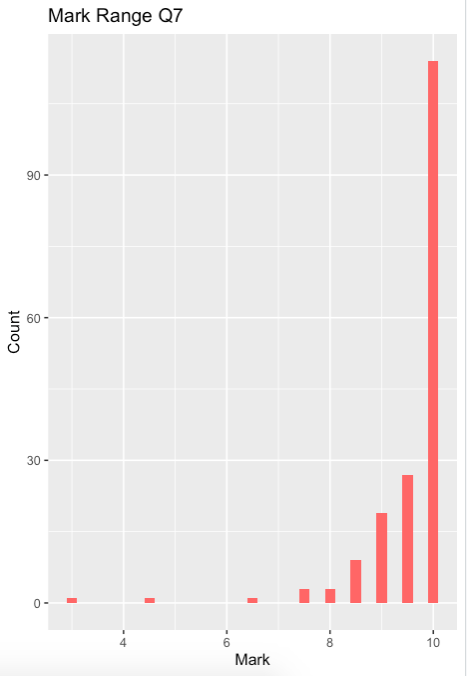
\includegraphics[scale=0.6]{Doc/q7-plot1.png}
    \caption{Phổ điểm của các sinh viên học đối phó}
    \label{fig:my_label}
\end{figure}
\\
\textbf{Câu 9: } 
\noindent Số sinh viên thông minh là: 285
\begin{figure}[!ht]
    \centering
    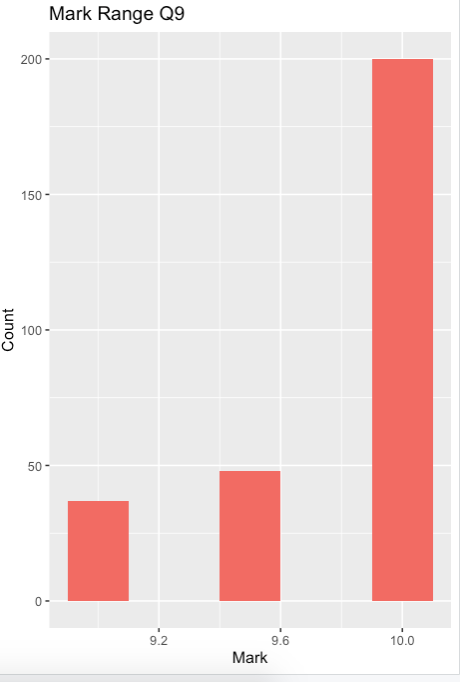
\includegraphics[scale=0.6]{Doc/q9-plot1.PNG}
    \caption{Phổ điểm của các sinh viên thông minh}
    \label{fig:my_label}
\end{figure}
\newpage
\subsection{File 2}
\textbf{Câu 1: }\\
\textbf{Câu 2: }\\
\textbf{Câu 3: }\\
\textbf{Câu 4: }\\
\textbf{Câu 5: }\\
\textbf{Câu 7: }\\
\noindent Số sinh viên học đối phó là: 197
\noindent $t_2$ = 2020-04-20 00:00:00
\begin{figure}[!ht]
    \centering
    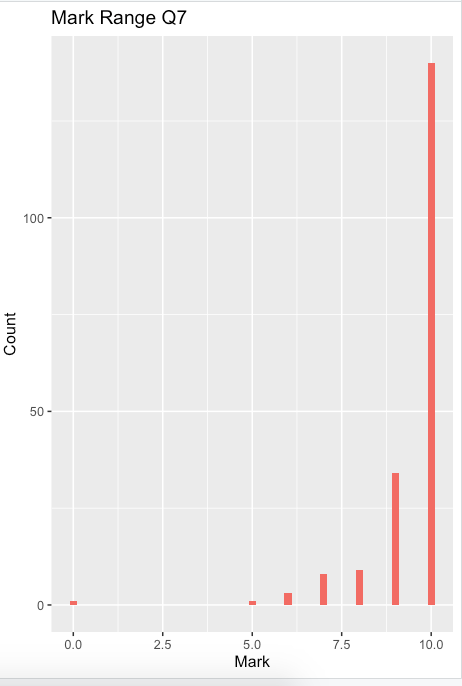
\includegraphics[scale=0.6]{Doc/q7-plot2.PNG}
    \caption{Phổ điểm của các sinh viên học đối phó}
    \label{fig:my_label}
\end{figure}
\\
\textbf{Câu 9: }\\
\noindent Số sinh viên thông minh là 250
\begin{figure}[!ht]
    \centering
    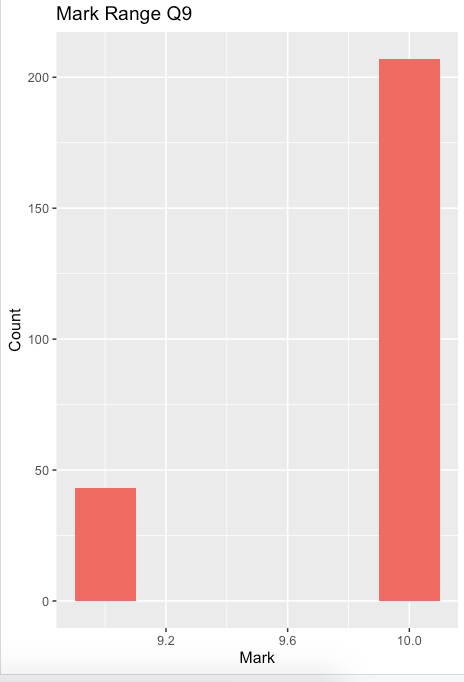
\includegraphics[scale=0.6]{Doc/q9-plot2.PNG}
    \caption{Phổ điểm các sinh viên thông minh}
    \label{fig:my_label}
\end{figure}
\newpage
\subsection{File 3}
\textbf{Câu 1: }\\
\textbf{Câu 2: }\\
\textbf{Câu 3: }\\
\textbf{Câu 4: }\\
\textbf{Câu 5: }\\
\textbf{Câu 7: }\\
\noindent Số sinh viên học đối phó là: 138
\noindent $t_2$ = 2020-04-24 00:00:00
\begin{figure}[!ht]
    \centering
    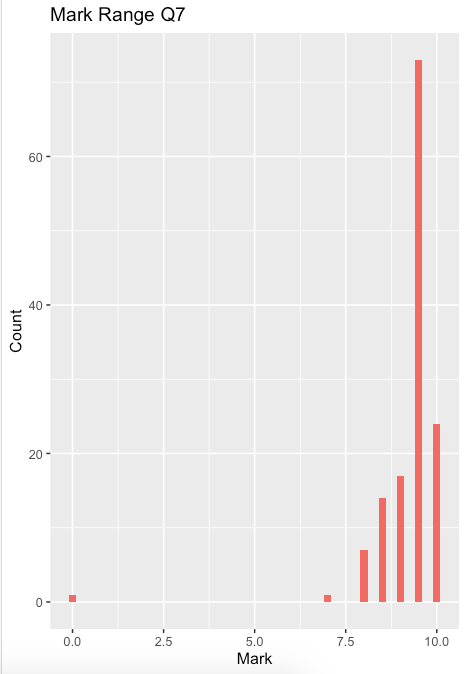
\includegraphics[scale=0.6]{Doc/q7-plot3.PNG}
    \caption{Phổ điểm các sinh viên học đối phó}
    \label{fig:my_label}
\end{figure}
\\
\textbf{Câu 9: }\\
\noindent Số sinh viên thông minh là: 250
\begin{figure}[!ht]
    \centering
    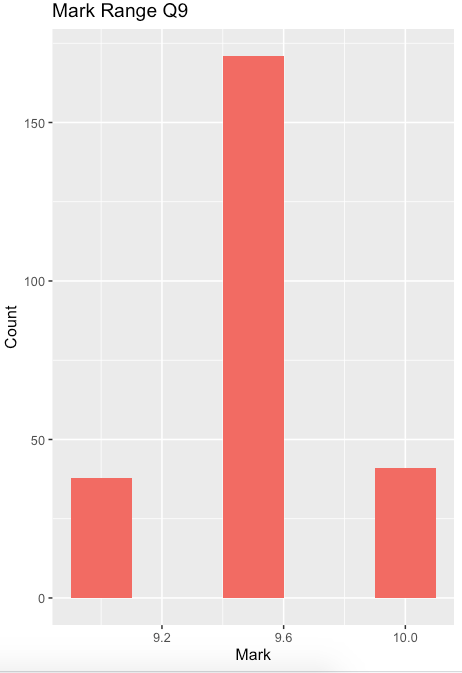
\includegraphics[scale=0.6]{Doc/q9-plot3.PNG}
    \caption{Phổ điểm các sinh viên thông minh}
    \label{fig:my_label}
\end{figure}
\newpage


\subsection{File 4}
\textbf{Câu 1: }\\
\textbf{Câu 2: }\\
\textbf{Câu 4: }\\
\textbf{Câu 3: }\\
\textbf{Câu 5: }\\
\textbf{Câu 7: }\\
\noindent Số sinh viên học đối phó là: 159
\noindent $t_2$ = 2020-04-18 00:00:00
\begin{figure}[!ht]
    \centering
    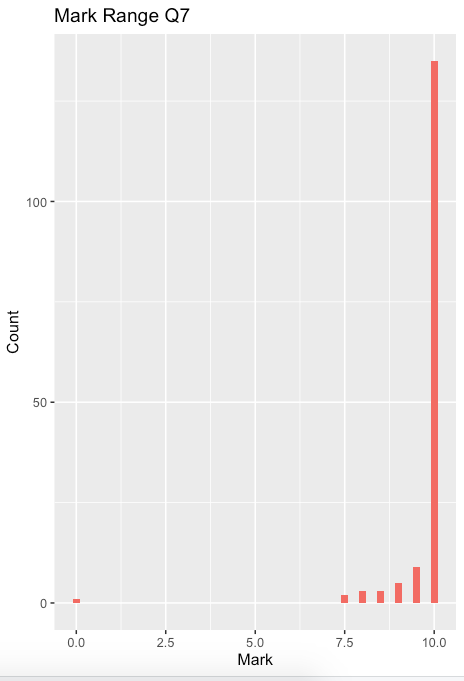
\includegraphics[scale=0.6]{Doc/q7-plot4.PNG}
    \caption{Phổ điểm các sinh viên học đối phó}
    \label{fig:my_label}
\end{figure}
\\
\textbf{Câu 9: }\\
\noindent Số sinh viên thông minh là: 298
\begin{figure}[!ht]
    \centering
    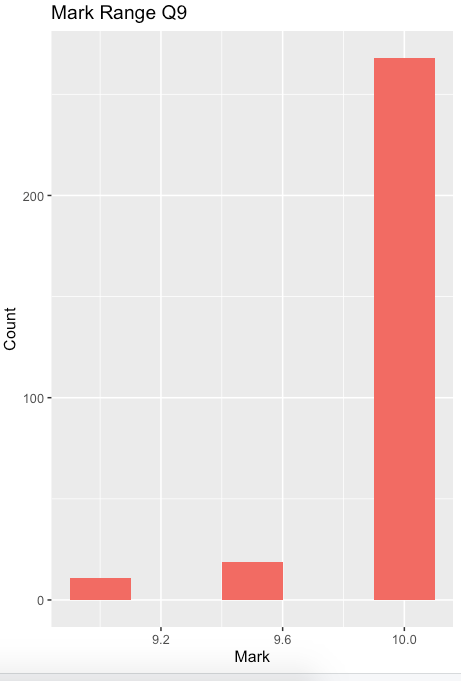
\includegraphics[scale=0.6]{Doc/q9-plot4.PNG}
    \caption{Phổ điểm các sinh viên thông minh}
    \label{fig:my_label}
\end{figure}
%Nguồn tham khảo
%--------------------------------------------------------
\newpage
\section{Nguồn tham khảo}
\begin{thebibliography}{80}


	\bibitem{GG} Google Images. Last access: 29/12/2019


	\bibitem{http://wikipedia:2019} Wikipedia.
	``\textbf{link: http://en.wikipedia.org/}'',
	Last access: 29/12/2019.
	
	
	
\end{thebibliography}	
\end{document}
